\documentclass{beamer}

\usepackage[utf8]{inputenc}

\usepackage{amsmath}
\usepackage{amssymb}
\usepackage{amsthm}
\usepackage{amsfonts}
\usepackage{xspace}
\usepackage{tabularx,booktabs,multirow}

\usepackage{hyperref}
\usepackage{url}

\usepackage{tikz}
\usepackage{color}
\usetikzlibrary{calc,shapes,fadings,automata,backgrounds,petri,shapes,decorations,decorations.pathmorphing,decorations.pathreplacing}


%%%%%%%%%% Tool Names %%%%%%%%%%%%
\newcommand{\pn}{Petri net}
\newcommand{\pns}{Petri nets}
\newcommand{\apical}{$A\pi$-calculus}
\newcommand{\pical}{$\pi$-calculus}
\newcommand{\nest}{\mathit{nest}_\nu}
\newcommand{\depth}{\mathit{depth}}
\newcommand{\set}[1]{\left\{#1\right\}}
\newcommand{\pset}[2]{\set{\,#1\mid#2\,}}
\newcommand{\process}{\mathcal{P}}
\newcommand{\Reach}{\mathit{Reach}}
\newcommand{\subgraph}{\mathrel{\hookrightarrow}}
\newcommand{\picasso}{\textsc{Picasso}\xspace}

\newcommand{\tikzMessage}[1]{
  \draw[thick,fill=white] (#1) rectangle ++(0.6, -0.4);
  \path[draw,-,thick] (#1) -- ++(0.3, -0.2) -- ++(0.3, 0.2); 
}
\newcommand{\tikzMessageNode}[2]{
  \node[draw,thick,fill=white,rectangle,inner sep=0pt,minimum height=0.4cm,minimum width=0.6cm] (#1) at (#2) {};
  \path[draw,-,thick] (#2) -- ++(-0.3, 0.2) (#2) -- ++(0.3, 0.2); 
}

\mode<presentation>
{
  \usetheme{Warsaw}
  \useoutertheme{mysplit}
}
% Remove the navigation bar
\setbeamertemplate{navigation symbols}{}

\AtBeginSubsection[]
{
  \begin{frame}
    \frametitle{Table of Contents}
    \tableofcontents[currentsection,currentsubsection]
  \end{frame}
}

\graphicspath{{./imgs/}}

\title[Analysis and Application of DBS]{Analysis and Application of Depth-Bounded Systems}

\author{Damien Zufferey}

\institute{
  IST Austria
}
\date{EPFL - LARA, 12.09.2012}

\begin{document}

% Title
\frame[plain]{\titlepage}

%\begin{frame}
%  \frametitle{What are Depth-Bounded Processes (DBP) ?}
%
%  \begin{description}
%  \item[As buzzwords:]
%  concurrent/distributed message-passing programs with process creation and mobility.\\
%  (Warning restrictions may apply.)
%  \item[For the programmers:] some class of programs using the actor model (Erlang, Scala, Akka, ActorFoundry, $\ldots$)
%  \item[For the theoreticians:] a fragment of the $\pi$-calculus.
%  \end{description}
%
%\end{frame}

\begin{frame}
  \frametitle{Outline}
  \tableofcontents
\end{frame}


\section{Where it all started}

\begin{frame}[fragile]
  \frametitle{Example (1): scala/docs/examples/actors/pingpong.scala}

  \begin{columns}
    \column{6cm}
{\tiny
\begin{verbatim}
class Ping(count: Int, pong: Actor) extends Actor {
  def act() {
    var pingsLeft = count - 1
    pong ! Ping
    loop {
      react {
        case Pong =>
          if (pingsLeft % 1000 == 0)
            println("Ping: pong")
          if (pingsLeft > 0) {
            pong ! Ping
            pingsLeft -= 1
          } else {
            println("Ping: stop")
            pong ! Stop
            exit()
          }
      }
    }
  }
}
\end{verbatim}
}

    \column{5cm}
{\tiny
\begin{verbatim}
class Pong extends Actor {
  def act() {
    var pongCount = 0
    loop {
      react {
        case Ping =>
          if (pongCount % 1000 == 0)
            println("Pong: ping "+pongCount)
          sender ! Pong
          pongCount += 1
        case Stop =>
          println("Pong: stop")
          exit()
      }
    }
  }
}
\end{verbatim}
}
  \end{columns}
\end{frame}

\begin{frame}
  \frametitle{Example (2): scala/docs/examples/actors/pingpong.scala}

  \begin{columns}
    \column{5cm}
    \begin{figure}[!ht]
      \centering
      \textbf{actor$_{ping}$}
      
      \vspace{10pt}
      
      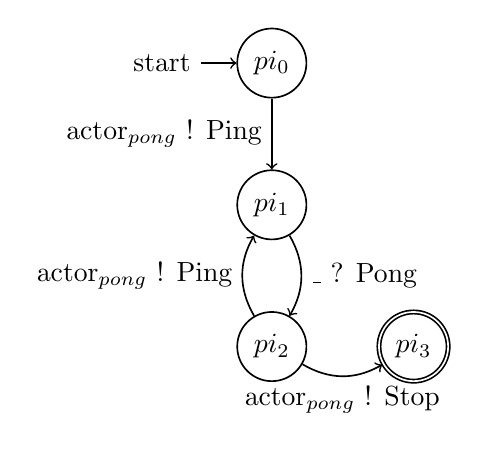
\begin{tikzpicture}[->,auto, node distance=18mm, semithick]
      \node [state,initial] (pi0) {$pi_0$};
      \node [state] (pi1) [below of=pi0] {$pi_1$};
      \node [state] (pi2) [below of=pi1] {$pi_2$};
      \node [state,accepting] (pi3) [right of=pi2] {$pi_3$};
      \path
      (pi0) edge node[left] { actor$_{pong}$ ! Ping } (pi1)
      (pi1) edge [bend left] node[right] { \_ ? Pong } (pi2)
      (pi2) edge [bend left] node[left] { actor$_{pong}$ ! Ping } (pi1)
      (pi2) edge [bend right] node[below] { actor$_{pong}$ ! Stop } (pi3)
      ;
      \end{tikzpicture}
    \end{figure}

    \column{5cm}
    \begin{figure}[!ht]
      \centering
      \textbf{actor$_{pong}$}
      
      \vspace{10pt}
      
      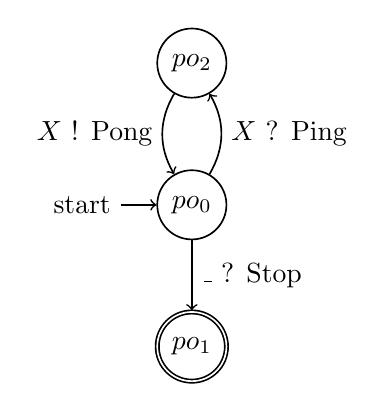
\begin{tikzpicture}[->,auto, node distance=18mm, semithick]
      \node [state,initial] (po0) {$po_0$};
      \node [state,accepting] (po1) [below of=po0] {$po_1$};
      \node [state] (po2) [above of=po0] {$po_2$};
      \path
      (po0) edge node[right] { \_ ? Stop } (po1)
      (po0) edge [bend right] node[right] { $X$ ? Ping } (po2)
      (po2) edge [bend right] node[left] { $X$ ! Pong} (po0)
      ;
      \end{tikzpicture}
    \end{figure}
  \end{columns}
\end{frame}

\begin{frame}
  \frametitle{Example: client-server communication pattern}
  \begin{figure}
  \centering
  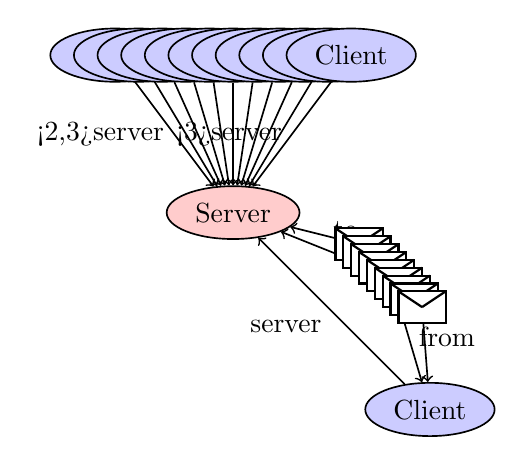
\begin{tikzpicture}[semithick, ->, node distance=2cm]
  \node [draw,ellipse,fill=red!20]  (x) at ( 0, 0) {Server};

  %replication of clients
  \visible<2-> {
  \node [draw,ellipse,fill=blue!20] (ni) at (-1.5, 2) {Client};
  \path  (ni) edge node [left] {\alt<2,3>{server}{}} (x);
  }

  \visible<4-> {
  \node [draw,ellipse,fill=blue!20] (n1) at (-1.2, 2) {Client};
  \path  (n1) edge (x);
  \node [draw,ellipse,fill=blue!20] (n2) at (-0.9, 2) {Client};
  \path  (n2) edge (x);
  \node [draw,ellipse,fill=blue!20] (n3) at (-0.6, 2) {Client};
  \path  (n3) edge (x);
  \node [draw,ellipse,fill=blue!20] (n4) at (-0.3, 2) {Client};
  \path  (n4) edge (x);
  \node [draw,ellipse,fill=blue!20] (n5) at ( 0  , 2) {Client};
  \path  (n5) edge (x);
  \node [draw,ellipse,fill=blue!20] (n6) at ( 0.3, 2) {Client};
  \path  (n6) edge (x);
  \node [draw,ellipse,fill=blue!20] (n7) at ( 0.6, 2) {Client};
  \path  (n7) edge (x);
  \node [draw,ellipse,fill=blue!20] (n8) at ( 0.9, 2) {Client};
  \path  (n8) edge (x);
  \node [draw,ellipse,fill=blue!20] (n9) at ( 1.2, 2) {Client};
  \path  (n9) edge (x);
  }

  \visible<3-> {
  \node [draw,ellipse,fill=blue!20] (nj) at ( 1.5, 2) {Client};
  \path  (nj) edge node [left] {\alt<3>{server}{}} (x);
  }
  
  %replication of messages
  \visible<5-> {
  \node [draw,ellipse,fill=blue!20] (m) at ( 2.5, -2.5) {Client};
  \path  (m) edge node [below left] {server} (x);
  }
  
  \visible<6> {
  \tikzMessageNode{mm}{2.0,-0.8}
  \path  (mm) edge node [right] {from} (m);
  \path  (mm) edge node [above right] {to} (x);
  }

  \visible<7-> {
  \tikzMessageNode{m1}{1.6,-0.4}
  \tikzMessageNode{m3}{1.7,-0.5}
  \tikzMessageNode{m4}{1.8,-0.6}
  \tikzMessageNode{m5}{1.9,-0.7}
  \tikzMessageNode{m6}{2.0,-0.8}
  \tikzMessageNode{m7}{2.1,-0.9}
  \tikzMessageNode{m8}{2.2,-1.0}
  \tikzMessageNode{m9}{2.3,-1.1}
  \tikzMessageNode{m2}{2.4,-1.2}
  \path  (m2) edge (m);
  \path  (m1) edge (x);
  }
  
  \end{tikzpicture}
  \end{figure}
\end{frame}


\begin{frame}
  \frametitle{What kind of properties are we looking at ?}
  Safety properties, more precisely the control-state reachability problem (aka covering problem).

  \begin{figure}
  \centering
  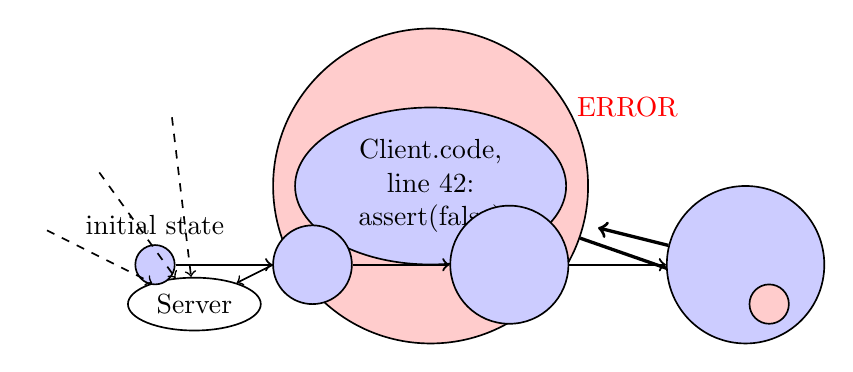
\begin{tikzpicture}[semithick, ->, node distance=2cm]

  \visible<1-2,8> {
  \node[draw,circle,fill=red!20, minimum height=4cm] (err1) at (-0.5,1) {} ;
  \node[color=red] (errlabel) at ( 2, 2) {ERROR};
  \node [draw,ellipse,fill=blue!20,text width=22mm, text centered]  (x) at ( -0.5, 1) {Client.code, line 42: assert(false)};
  \visible<8> {
  \node [draw,ellipse]  (server) at ( -3.5, -0.5) {Server};
  \path  (x) edge (server);
  }
  }

  \visible<2-5> {
  \node[draw,circle,fill=red!20,minimum height=0.5cm]  (err2) at ( 3.8, -0.5) {};
  }
  \visible<2> {
  \path[very thick] (err1) edge (err2);
  }
  \visible<3-6> {
  \node[draw,circle,fill=blue!20,minimum height=0.5cm]  (init) at ( -4, 0) {};
  }
  \visible<3> {
  \node (initlabel) at ( -4, 0.5) {initial state};
  }
  \visible<4-6> {
  \node[draw,circle,fill=blue!20,minimum height=1cm]  (s1) at ( -2, 0) {};
  \path[thick] (init) edge (s1);
  }
  \visible<5-6> {
  \node[draw,circle,fill=blue!20,minimum height=1.5cm]  (s2) at ( 0.5, 0) {};
  \path[thick] (s1) edge (s2);
  }
  \visible<6-8> {
  \node[draw,circle,fill=blue!20,minimum height=2cm]  (s3) at ( 3.5, 0) {};
  \visible<6>{\path[thick] (s2) edge (s3);}
  \node[draw,circle,fill=red!20,minimum height=0.5cm]  (err2) at ( 3.8, -0.5) {};
  }
  \visible<8> {
  \node (invisible) at (1.5,0.5) {};
  \path[very thick] (s3) edge (invisible);
  \begin{scope}
  \node (cli1) at (-3.8,2) {};
  \node (cli2) at (-4.8,1.3) {};
  \node (cli3) at (-5.5,0.5) {};
  \path [dashed] (cli1) edge (server);
  \path [dashed] (cli2) edge (server);
  \path [dashed] (cli3) edge (server);
  \end{scope}
  }

  \end{tikzpicture}
  \end{figure}

\end{frame}

\begin{frame}
  \frametitle{Depth-bounded systems: \cite{Meyer08OnBoundednessInDepth}}
  System with a bound on the longest acyclic path.\\
  (Concretely: it is not possible to encode an infinite memory.)

  \vspace{10pt}

  \begin{figure}
  \centering
  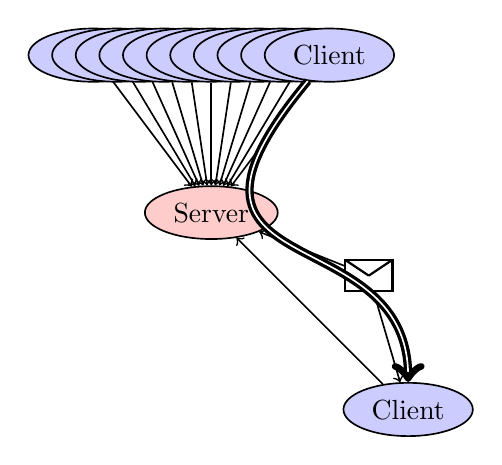
\begin{tikzpicture}[semithick, ->, node distance=2cm]
  \node [draw,ellipse,fill=red!20]  (x) at ( 0, 0) {Server};

  \node [draw,ellipse,fill=blue!20] (ni) at (-1.5, 2) {Client};
  \path  (ni) edge node [left] {} (x);
  \node [draw,ellipse,fill=blue!20] (n1) at (-1.2, 2) {Client};
  \path  (n1) edge (x);
  \node [draw,ellipse,fill=blue!20] (n2) at (-0.9, 2) {Client};
  \path  (n2) edge (x);
  \node [draw,ellipse,fill=blue!20] (n3) at (-0.6, 2) {Client};
  \path  (n3) edge (x);
  \node [draw,ellipse,fill=blue!20] (n4) at (-0.3, 2) {Client};
  \path  (n4) edge (x);
  \node [draw,ellipse,fill=blue!20] (n5) at ( 0  , 2) {Client};
  \path  (n5) edge (x);
  \node [draw,ellipse,fill=blue!20] (n6) at ( 0.3, 2) {Client};
  \path  (n6) edge (x);
  \node [draw,ellipse,fill=blue!20] (n7) at ( 0.6, 2) {Client};
  \path  (n7) edge (x);
  \node [draw,ellipse,fill=blue!20] (n8) at ( 0.9, 2) {Client};
  \path  (n8) edge (x);
  \node [draw,ellipse,fill=blue!20] (n9) at ( 1.2, 2) {Client};
  \path  (n9) edge (x);
  \node [draw,ellipse,fill=blue!20] (nj) at ( 1.5, 2) {Client};
  \path  (nj) edge node [left] {} (x);
  
  \node [draw,ellipse,fill=blue!20] (m) at ( 2.5, -2.5) {Client};
  \path  (m) edge node [below left] {} (x);
  
  \tikzMessageNode{mm}{2.0,-0.8}
  \path  (mm) edge node [right] {} (m);
  \path  (mm) edge node [above right] {} (x);

  \draw[very thick,double] (nj) .. controls (-1,-1) and (2.5,0) .. (m);

  \end{tikzpicture}
  \end{figure}
\end{frame}


%\section{Formalism}
\begin{frame}
  \frametitle{Formal model: WSTS}
  A well-structured transition system (WSTS)
  is a transition system $\langle S, \rightarrow, \leq \rangle$ such that:
  \begin{itemize}
  \item
    $\leq$ is a well-quasi-ordering (wqo),\\
    i.e. well-founded + no infinite antichain.
  \item
    compatibility of $\leq$ w.r.t. $\rightarrow$\\
    \begin{center}
    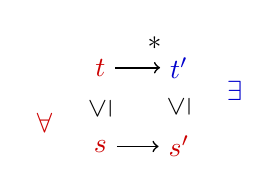
\begin{tikzpicture}[semithick, ->]
    \node[color=red!80!black] (s) {$s$};
    \node[color=red!80!black] (t) [above of=s] {$t$};
    \node[color=red!80!black] (sp) [right of=s] {$s'$};
    \node[color=blue!80!black] (tp) [right of=t] {$t'$};

    \path[color=white]  (s) edge node[color=black,rotate=90] {$\leq$} (t);
    \path  (s) edge (sp);
    \path  (t) edge node [above right] {*} (tp);
    \path[color=white]  (sp) edge node[color=black,rotate=90] {$\leq$} (tp);
    
    \node[color=blue!80!black] (exists) [above right of=sp] {$\exists$};
    \node[color=red!80!black] (forall) [below left of=t] {$\forall$};

    \end{tikzpicture}
    \end{center}
  \end{itemize}

  For more detail see: \cite{DBLP:journals/tcs/FinkelS01, DBLP:conf/lics/AbdullaCJT96}

\end{frame}

\begin{frame}
  \frametitle{Downward Closure}
  \begin{figure}
  \centering
  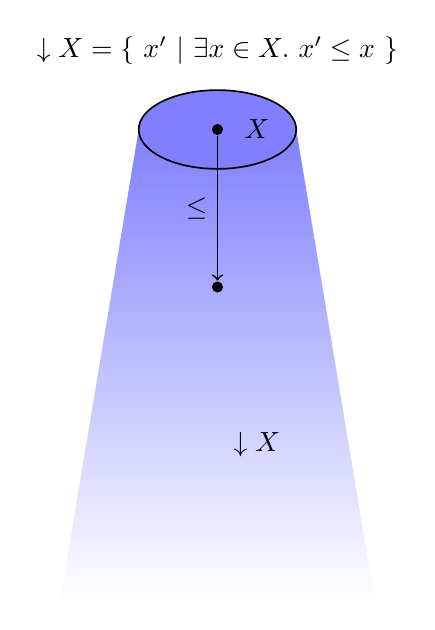
\begin{tikzpicture}[semithick, ->, node distance=2cm]

    \node at (-2,4) {$\downarrow X = \{~ x' ~|~ \exists x \in X.~ x' \leq x ~\}$};
    \shade[top color=blue!50,bottom color=white] (0,-3) -- (-1,3) -- (-3,3) -- (-4,-3);
    \node[draw,ellipse,fill=blue!50,minimum height=1cm,minimum width=2cm] at (-2,3) {};
    \node at (-1.5,3) {$X$};
    \node at (-1.5,-1) {$\downarrow X$};
    \node[fill=black,circle,inner sep=0pt,minimum size=4pt] (d1) at (-2,3) {};
    \node[fill=black,circle,inner sep=0pt,minimum size=4pt] (d2) at (-2,1) {};
    \path (d1) edge node[left] {$\leq$} (d2);
    
  \end{tikzpicture}
  \end{figure}
\end{frame}

\begin{frame}
  \frametitle{Forward algorithm for covering}
  \begin{center}
  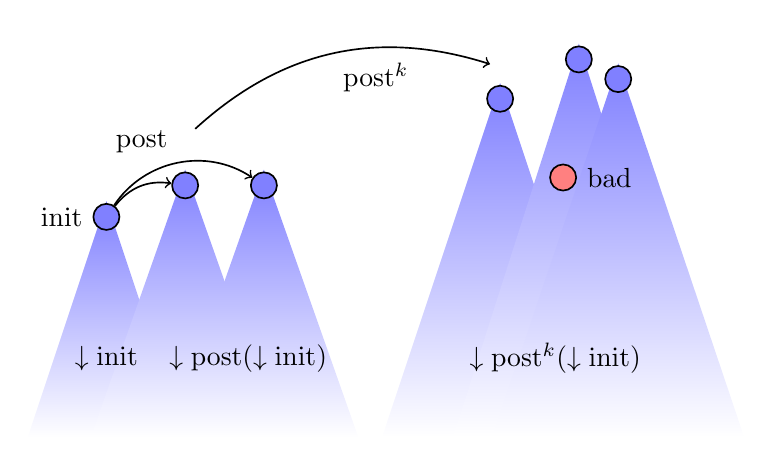
\begin{tikzpicture}[semithick,->]

  \shade[top color=blue!50,bottom color=white] (-3,-5) -- (-4,-2) -- (-5,-5);
  \node[draw,circle,fill=blue!50,minimum height=0.2,label={left:init}] (e1) at (-4,-2.2) {};

  \visible<2->{
  \shade[top color=blue!50,bottom color=white] (-1.8,-5) -- (-3,-1.6) -- (-4.2,-5);
  \node[draw,circle,fill=blue!50,minimum height=0.2] (e2) at (-3,-1.8) {};
  \shade[top color=blue!50,bottom color=white] (-0.8,-5) -- (-2,-1.6) -- (-3.2,-5);
  \node[draw,circle,fill=blue!50,minimum height=0.2] (e3) at (-2,-1.8) {};
  \path (e1) edge[bend left] (e2);
  \path (e1) edge[bend left=45] node[above left] {post} (e3);
  \node at (-2.2,-4) {$\downarrow\text{post}(\downarrow\text{init})$};
  }

  \visible<3->{
  \shade[top color=blue!50,bottom color=white] (2.5,-5) -- (1,-0.5) -- (-0.5,-5);
  \node[draw,circle,fill=blue!50,minimum height=0.2] at (1,-0.7) {};
  \shade[top color=blue!50,bottom color=white] (3.6,-5) -- (2,0) -- (0.4,-5);
  \node[draw,circle,fill=blue!50,minimum height=0.2] at (2,-0.2) {};
  \shade[top color=blue!50,bottom color=white] (4.1,-5) -- (2.5,-0.25) -- (0.9,-5);
  \node[draw,circle,fill=blue!50,minimum height=0.2] at (2.5,-0.45) {};

  \node (e4) at (-3,-1.2) {};
  \node (e5) at (1,-0.3) {};
  \path (e4) edge[bend left] node[below right] {post$^k$} (e5);
  \node at (1.7,-4) {$\downarrow\text{post}^k(\downarrow\text{init})$};
  }

  \visible<4->{
  \node[draw,circle,fill=red!50,minimum height=0.2,label={right:bad}] at (1.8,-1.7) {};
  }
  %on top of the shades
  \node at (-4,-4) {$\downarrow\text{init}$};
  \end{tikzpicture}
  \end{center}
  \visible<5->{
      Computes the covering set rather than answering only a single coverability query.
  }
\end{frame}

%TODO issues for analyzing the ...

\section{Computing the Covering Set for DBS}

%introduce the concept of ideal: 
\begin{frame}
  \frametitle{Representing downward-closed sets with ideals}

  
  \begin{minipage}{0.5\linewidth}
  Given a wqo-set $(X,\leq)$.

  \vspace{10pt}

  A subset of $X$ is \alert{directed} if it is non-empty and closed under upper bounds.
  
  \vspace{10pt}

  An \alert{ideal} of $X$ is a directed downward-closed subset of X.
  
  \vspace{10pt}

  The ideal completion $Idl(X)$ of $X$ is the set of all ideals of $X$.
  \end{minipage}
  \hspace{20pt}
  \begin{minipage}{0.4\linewidth}
  A downward-closed subset is a finite union of ideals.

  \vspace{10pt}

  \begin{center}
  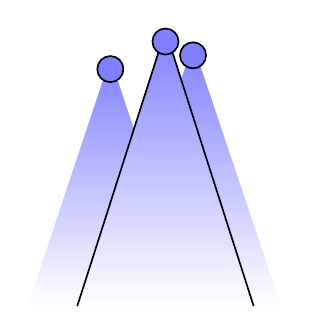
\begin{tikzpicture}[semithick,scale=0.7]
  \shade[top color=blue!50,bottom color=white] (2.5,-5) -- (1,-0.5) -- (-0.5,-5);
  \node[draw,circle,fill=blue!50,minimum height=0.2] at (1,-0.7) {};
  \shade[top color=blue!50,bottom color=white] (4.1,-5) -- (2.5,-0.25) -- (0.9,-5);
  \node[draw,circle,fill=blue!50,minimum height=0.2] at (2.5,-0.45) {};
  \shade[top color=blue!50,bottom color=white] (3.6,-5) -- (2,0) -- (0.4,-5);
  \path[draw] (3.6,-5) -- (2,0) -- (0.4,-5);
  \node[draw,circle,fill=blue!50,minimum height=0.2] at (2,-0.2) {};
  \end{tikzpicture}
  \end{center}
  \end{minipage}
\end{frame}

\begin{frame}
  \frametitle{Ideal for representing downward-closed sets.}
  ADL: \cite{GeeraertsETAL06ExpandEnlargeCheck}\\
  Further developed in \cite{FinkelGoubaultLarrecq09ForwardAnalysisForWSTS}\\
  Applied to DBP in \cite{WiesETAL10ForwardAnalysisofDepthBoundedProcesses}

  \begin{figure}
  \centering
  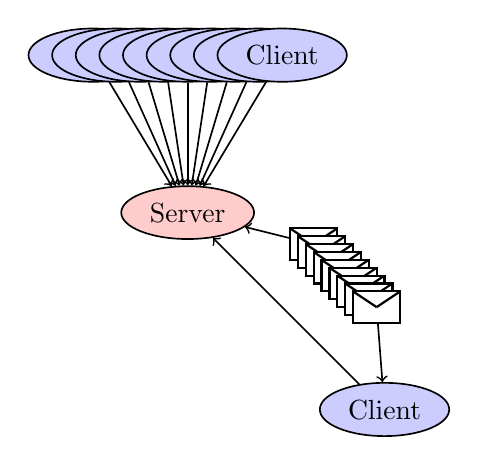
\begin{tikzpicture}[semithick, ->, node distance=2cm]
  \node [draw,ellipse,fill=red!20]  (x) at ( 0, 0) {Server};

  \node [draw,ellipse,fill=blue!20] (n1) at (-1.2, 2) {Client};
  \path  (n1) edge (x);
  \node [draw,ellipse,fill=blue!20] (n2) at (-0.9, 2) {Client};
  \path  (n2) edge (x);
  \node [draw,ellipse,fill=blue!20] (n3) at (-0.6, 2) {Client};
  \path  (n3) edge (x);
  \node [draw,ellipse,fill=blue!20] (n4) at (-0.3, 2) {Client};
  \path  (n4) edge (x);
  \node [draw,ellipse,fill=blue!20] (n5) at ( 0  , 2) {Client};
  \path  (n5) edge (x);
  \node [draw,ellipse,fill=blue!20] (n6) at ( 0.3, 2) {Client};
  \path  (n6) edge (x);
  \node [draw,ellipse,fill=blue!20] (n7) at ( 0.6, 2) {Client};
  \path  (n7) edge (x);
  \node [draw,ellipse,fill=blue!20] (n8) at ( 0.9, 2) {Client};
  \path  (n8) edge (x);
  \node [draw,ellipse,fill=blue!20] (n9) at ( 1.2, 2) {Client};
  \path  (n9) edge (x);

  \node [draw,ellipse,fill=blue!20] (m) at ( 2.5, -2.5) {Client};
  \path  (m) edge (x);
  
  \tikzMessageNode{m1}{1.6,-0.4}
  \tikzMessageNode{m3}{1.7,-0.5}
  \tikzMessageNode{m4}{1.8,-0.6}
  \tikzMessageNode{m5}{1.9,-0.7}
  \tikzMessageNode{m6}{2.0,-0.8}
  \tikzMessageNode{m7}{2.1,-0.9}
  \tikzMessageNode{m8}{2.2,-1.0}
  \tikzMessageNode{m9}{2.3,-1.1}
  \tikzMessageNode{m2}{2.4,-1.2}
  \path  (m2) edge (m);
  \path  (m1) edge (x);

  \end{tikzpicture}
  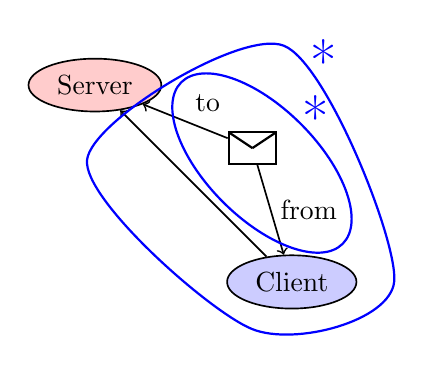
\begin{tikzpicture}[semithick, ->, node distance=2cm]
  \node [draw,ellipse,fill=red!20]  (x) at ( 0, 0) {Server};

  \node [draw,ellipse,fill=blue!20] (m) at ( 2.5, -2.5) {Client};
  \path  (m) edge (x);
  
  \tikzMessageNode{mm}{2.0,-0.8}
  \path  (mm) edge node [right] {from} (m);
  \path  (mm) edge node [above right] {to} (x);

  \draw[thick,rotate=45,color=blue] (0.8,-2.2) ellipse (0.7 and 1.45);
  \node[text=blue] (star) at ( 2.8, -0.4) {{\huge *}};

  \draw[color=blue,thick] plot[smooth cycle] coordinates{(-0.1,-0.95) (2.4,0.5) (3.8,-2.5) (2,-3.1)};
  \node[text=blue] (star) at ( 2.9, 0.3) {{\huge *}};

  \end{tikzpicture}
  \end{figure}
\end{frame}

\begin{frame}
  \frametitle{When does acceleration work ? (flat systems)}

  Forward algorithms are (usually) based on acceleration.

  Acceleration \emph{executes} loops infinitely many time (saturation).

  \vspace{10pt}

  Concretely, The algorithm terminates if the covering set can be generated by executing only simple loops.
  This condition is known as flattability \cite{DBLP:conf/atva/BardinFLS05}.
  Acceleration \emph{executes} traces of length $< \omega^2$.


  
  \begin{figure}
  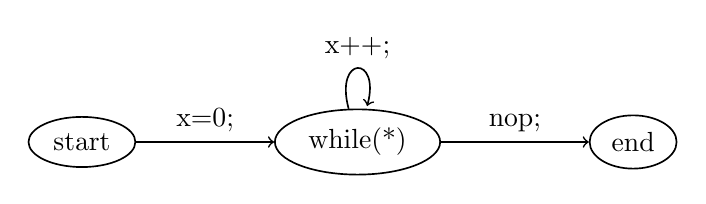
\begin{tikzpicture}[semithick, ->, node distance=35mm]

  \node [draw,ellipse] (loc1) at ( 0, 0) {start};
  \node [draw,ellipse] (loc2) [right of=loc1] {while(*)};
  \node [draw,ellipse] (loc3) [right of=loc2] {end};
  \path  (loc1) edge node[above] {x=0;} (loc2);
  \path  (loc2) edge [loop above] node[above] {x++;}(loc2);
  \path  (loc2) edge node[above] {nop;} (loc3);
  \end{tikzpicture}
  \caption{Example of a flat program}
  \end{figure}

\end{frame}


\begin{frame}
  \frametitle{DBP are intrinsically non-flat.}

  \begin{minipage}{0.6\linewidth}
  initial configuration:
  
  \begin{figure}
  \centering
  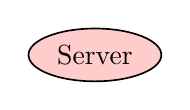
\begin{tikzpicture}[semithick, ->, node distance=2cm]
  \node [draw,ellipse,fill=red!20]  (x) at ( 0, 0) {Server};
  \end{tikzpicture}
  \end{figure}

  covering set:

  \begin{figure}
  \centering
  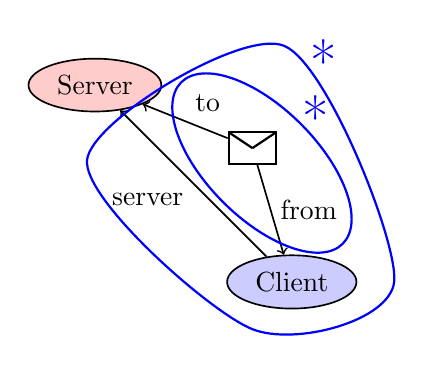
\begin{tikzpicture}[semithick, ->, node distance=2cm]
  \node [draw,ellipse,fill=red!20]  (x) at ( 0, 0) {Server};

  \node [draw,ellipse,fill=blue!20] (m) at ( 2.5, -2.5) {Client};
  \path  (m) edge node [below left] {server} (x);
  
  \tikzMessageNode{mm}{2.0,-0.8}
  \path  (mm) edge node [right] {from} (m);
  \path  (mm) edge node [above right] {to} (x);

  \draw[thick,rotate=45,color=blue] (0.8,-2.2) ellipse (0.7 and 1.45);
  \node[text=blue] (star) at ( 2.8, -0.4) {{\huge *}};

  \draw[color=blue,thick] plot[smooth cycle] coordinates{(-0.1,-0.95) (2.4,0.5) (3.8,-2.5) (2,-3.1)};
  \node[text=blue] (star) at ( 2.9, 0.3) {{\huge *}};

  \end{tikzpicture}
  \end{figure}
  
  \end{minipage}
  \begin{minipage}{0.35\linewidth}
  $\omega^2$ steps from the initial state and the final state.

  \vspace{10pt}

  Nested loops are required to compute the covering set.
  \end{minipage}

\end{frame}

%\section{Ideal Abstraction}
\begin{frame}
  \frametitle{From acceleration to widening}

  Acceleration considers transitions - widening only states.

  \begin{figure}
  \centering
  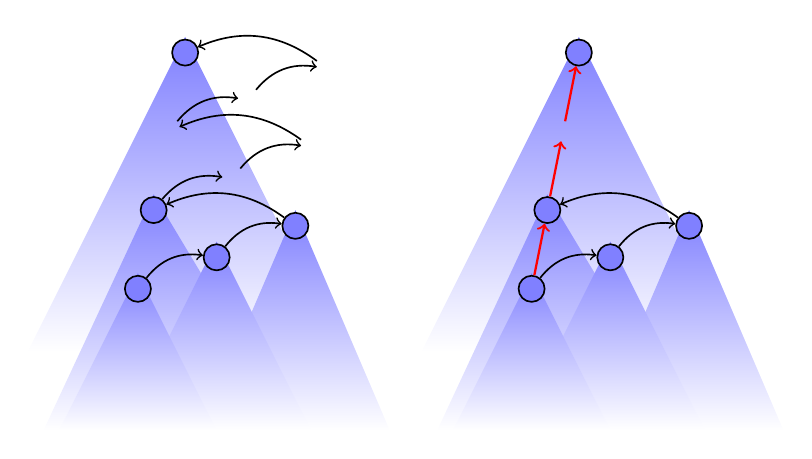
\begin{tikzpicture}[semithick, ->, node distance=2cm]

  \begin{scope}
  
  %layer 1: shades
  \visible<6->{
    \shade[top color=blue!50,bottom color=white] (-1.4,-3) -- (-3.4,1) -- (-5.4,-3);
  }
  \visible<5->{
  }
  \visible<4->{
    \shade[top color=blue!50,bottom color=white] (-2,-4) -- (-3.8,-1.0) -- (-5.2,-4);
  }
  \visible<3->{
    \shade[top color=blue!50,bottom color=white] (-0.8,-4) -- (-2,-1.2) -- (-3.2,-4);
  }
  \visible<2->{
    \shade[top color=blue!50,bottom color=white] (-1.8,-4) -- (-3,-1.6) -- (-4.2,-4);
  }
  \visible<1->{
    \shade[top color=blue!50,bottom color=white] (-3,-4) -- (-4,-2) -- (-5,-4);
  }
  
  %layer 2: nodes
  \visible<1->{
    \node[draw,circle,fill=blue!50] (e1) at (-4,-2.2) {};
  }
  \visible<2->{
    \node[draw,circle,fill=blue!50] (e2) at (-3,-1.8) {};
  }
  \visible<3->{
    \node[draw,circle,fill=blue!50] (e3) at (-2,-1.4) {};
  }
  \visible<4->{
    \node[draw,circle,fill=blue!50] (e4) at (-3.8,-1.2) {};
  }
  \visible<5->{
    \node (e5) at (-2.8,-0.8) {};
    \node (e6) at (-1.8,-0.4) {};
    \node (e7) at (-3.6,-0.2) {};
  }
  \visible<6->{
    \node (e8) at (-2.6,0.2) {};
    \node (e9) at (-1.6,0.6) {};
    \node[draw,circle,fill=blue!50] (e10) at (-3.4,0.8) {};
  }

  %layer 3: edges 
  \visible<1->{
  }
  \visible<2->{
    \path (e1) edge[bend left] (e2);
  }
  \visible<3->{
    \path (e2) edge[bend left] (e3);
  }
  \visible<4->{
    \path (e3) edge[bend right] (e4);
  }
  \visible<5->{
    \path (e4) edge[bend left] (e5);
    \path (e5) edge[bend left] (e6);
    \path (e6) edge[bend right] (e7);
  }
  \visible<6->{
    \path (e7) edge[bend left] (e8);
    \path (e8) edge[bend left] (e9);
    \path (e9) edge[bend right] (e10);
  }
  
  \end{scope}
  
  \begin{scope}[xshift=5cm]
  
  %layer 1: shades
  \visible<12->{
    \shade[top color=blue!50,bottom color=white] (-1.4,-3) -- (-3.4,1) -- (-5.4,-3);
  }
  \visible<11->{
  }
  \visible<10->{
    \shade[top color=blue!50,bottom color=white] (-2,-4) -- (-3.8,-1.0) -- (-5.2,-4);
  }
  \visible<9->{
    \shade[top color=blue!50,bottom color=white] (-0.8,-4) -- (-2,-1.2) -- (-3.2,-4);
  }
  \visible<8->{
    \shade[top color=blue!50,bottom color=white] (-1.8,-4) -- (-3,-1.6) -- (-4.2,-4);
  }
  \visible<7->{
    \shade[top color=blue!50,bottom color=white] (-3,-4) -- (-4,-2) -- (-5,-4);
  }
  
  %layer 2: nodes
  \visible<7->{
    \node[draw,circle,fill=blue!50] (e1) at (-4,-2.2) {};
  }
  \visible<8->{
    \node[draw,circle,fill=blue!50] (e2) at (-3,-1.8) {};
  }
  \visible<9->{
    \node[draw,circle,fill=blue!50] (e3) at (-2,-1.4) {};
  }
  \visible<10->{
    \node[draw,circle,fill=blue!50] (e4) at (-3.8,-1.2) {};
  }
  \visible<11->{
  }
  \visible<12->{
    \node (e7) at (-3.6,-0.2) {};
    \node[draw,circle,fill=blue!50] (e10) at (-3.4,0.8) {};
  }

  %layer 3: edges 
  \visible<7->{
  }
  \visible<8->{
    \path (e1) edge[bend left] (e2);
  }
  \visible<9->{
    \path (e2) edge[bend left] (e3);
  }
  \visible<10->{
    \path (e3) edge[bend right] (e4);
  }
  \visible<11->{
    \path (e1) edge[red,thick] (e4);
  }
  \visible<12->{
    \path (e4) edge[red,thick] (e7);
    \path (e7) edge[red,thick] (e10);
  }
  
  \end{scope}

  \end{tikzpicture}
  \end{figure}

\end{frame}

\begin{frame}
  \frametitle{Ideal abstraction}

  Rephrase analysis in terms of abstract interpretation \cite{CousotCousot77AbstractInterpretation}.

  \begin{itemize}
  \item Concrete domain: sets of configurations ($\mathcal{P}(S)$)
  \item Abstract domain: \alert{ideal completion of $(S,\leq)$} ($\mathcal{P}_{finite}(Idl(S))$)
  \end{itemize}

  \vspace{5pt}

  \begin{itemize}
  \item Concretization function $\gamma$: identity
  \item Abstraction function $\alpha$: \alert{downward-closure}
  \end{itemize}
  $(\alpha,\gamma)$ is a Galois connection.

  \vspace{10pt}

  Covering set is abstract fixed point: $\mu X. \alpha(init) \cup \alpha \cdot post \cdot \gamma (X) $

  \vspace{5pt}

  To guarantee termination we need a widening operator.

\end{frame}

\begin{frame}
  \frametitle{Widening (1)}

  Goal: try to mimic acceleration (when possible), and force termination
  
  \vspace{1ex}

  A set-widening operator ($\nabla$) \cite{CousotCousot92AbstractInterpretationFrameworks} for a poset $S$ is partial function ($\mathcal{P}(S) \rightarrow S$) that satisfies:
  \begin{description}
  \item[Covering]: for all $X \subseteq S$, $x \in X \Rightarrow x \leq \nabla(X)$;
  \item[Termination]: widening of any ascending chain stabilizes.
  \end{description}

  \vspace{1ex}
  Why set-widening rather than the usual pair-widening.

  Reason of using a set-widening operator: we need the history.

\end{frame}

\begin{frame}
  \frametitle{Widening (2)}

  Keeping it simple: need only \alert{set-widening operator on $\mathit{Idl}(S)$}.
  
  It can be lifted to $\mathcal{P}_{finite}(Idl(S))$, using a general construction (details in the paper).

  \vspace{1ex}
  
  We assume that the ordering $S$ is a \alert{better-quasi-ordering} (bqo).\\
  $\Rightarrow$~ Thus, $\mathit{Idl}(S)$ is also a bqo.\\
  $\Rightarrow$~ No infinite antichain in $\mathit{Idl}(S)$.

  \vspace{1ex}
  
  We still need to define the widening on ideals.

  \vspace{1ex}

  We provide concrete operators for
  \begin{itemize}
  \item Petri nets (and monotonic extensions),
  \item Lossy channel systems \cite{DBLP:conf/lics/AbdullaJ93},
  \item Depth-bounded processes (DBP).
  \end{itemize}

\end{frame}

\begin{frame}
  \frametitle{Set-widening for DBP (1)}

  \begin{figure}
  \centering
  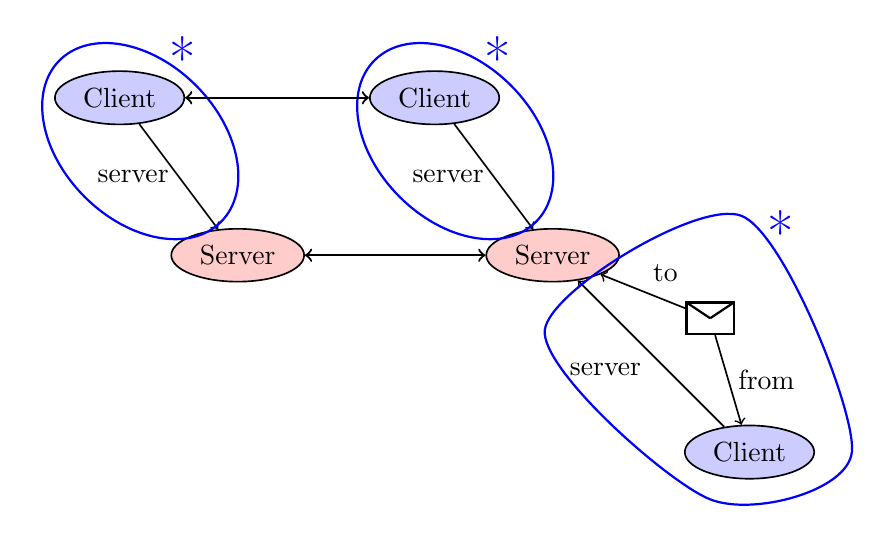
\begin{tikzpicture}[semithick, ->, node distance=2cm]


  \begin{scope}
    \node [draw,ellipse,fill=red!20]  (x) at ( 0, 0) {Server};
    \node [draw,ellipse,fill=blue!20] (ni) at (-1.5, 2) {Client};
    \path  (ni) edge node [left] {server} (x);
    \draw[thick,rotate=45,color=blue] (0.15,1.9) ellipse (1 and 1.45);
    \node[text=blue] (star) at ( -0.7, 2.5) {{\huge *}};
  \end{scope}
  
  \begin{scope}[xshift=4cm]
    \node [draw,ellipse,fill=red!20]  (x2) at ( 0, 0) {Server};
    \node [draw,ellipse,fill=blue!20] (ni2) at (-1.5, 2) {Client};
    \path  (ni2) edge node [left] {server} (x2);
    \draw[thick,rotate=45,color=blue] (0.15,1.9) ellipse (1 and 1.45);
    \node[text=blue] (star) at ( -0.7, 2.5) {{\huge *}};
    \node [draw,ellipse,fill=blue!20] (m) at ( 2.5, -2.5) {Client};
    \path  (m) edge node [below left] {server} (x2);
    \tikzMessageNode{mm}{2.0,-0.8}
    \path  (mm) edge node [right] {from} (m);
    \path  (mm) edge node [above right] {to} (x2);
  \end{scope}
  
  \visible<2->{
    \path[<->,thick] (x) edge (x2);
    \path[<->,thick] (ni) edge (ni2);
  }
  \visible<3->{
    \draw[color=blue,thick] plot[smooth cycle] coordinates{(3.9,-0.95) (6.4,0.5) (7.8,-2.5) (6,-3.1)};
    \node[text=blue] (star) at ( 6.9, 0.3) {{\huge *}};
  }

  \end{tikzpicture}
  \end{figure}
\end{frame}

\begin{frame}
  \frametitle{Set-widening for DBP (2)}

  \begin{figure}
  \centering
  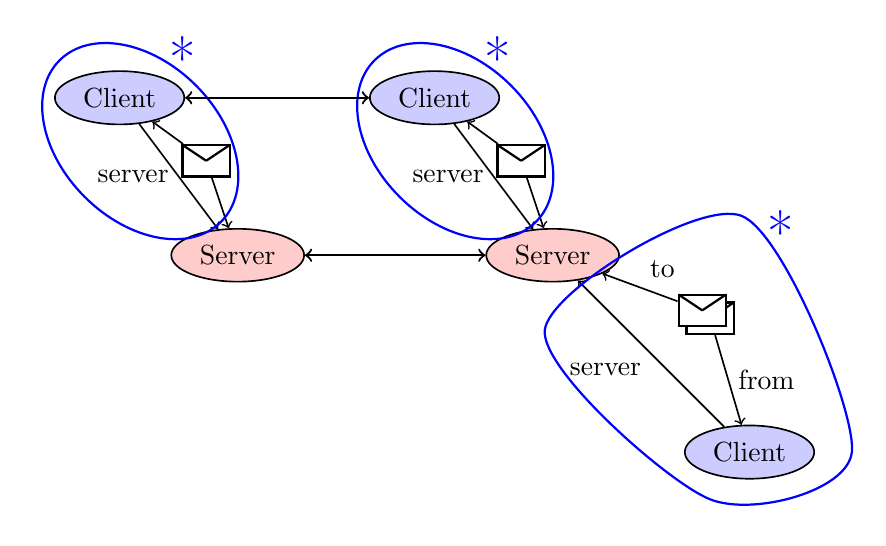
\begin{tikzpicture}[semithick, ->, node distance=2cm]

  \begin{scope}
    \node [draw,ellipse,fill=red!20]  (x) at ( 0, 0) {Server};
    \node [draw,ellipse,fill=blue!20] (ni) at (-1.5, 2) {Client};
    \path  (ni) edge node [left] {server} (x);
    \tikzMessageNode{om}{-0.4,1.2}
    \path  (om) edge (x);
    \path  (om) edge (ni);
    \draw[thick,rotate=45,color=blue] (0.15,1.9) ellipse (1 and 1.45);
    \node[text=blue] (star) at ( -0.7, 2.5) {{\huge *}};
  \end{scope}
  
  \begin{scope}[xshift=4cm]
    \node [draw,ellipse,fill=red!20]  (x2) at ( 0, 0) {Server};
    \node [draw,ellipse,fill=blue!20] (ni2) at (-1.5, 2) {Client};
    \path  (ni2) edge node [left] {server} (x2);
    \tikzMessageNode{om2}{-0.4,1.2}
    \path  (om2) edge (x2);
    \path  (om2) edge (ni2);
    \draw[thick,rotate=45,color=blue] (0.15,1.9) ellipse (1 and 1.45);
    \node[text=blue] (star) at ( -0.7, 2.5) {{\huge *}};
    \node [draw,ellipse,fill=blue!20] (m) at ( 2.5, -2.5) {Client};
    \path  (m) edge node [below left] {server} (x2);
    \tikzMessageNode{mm}{2.0,-0.8}
    \tikzMessageNode{mm2}{1.9,-0.7}
    \path  (mm) edge node [right] {from} (m);
    \path  (mm2) edge node [above right] {to} (x2);
  \end{scope}
  
  \visible<2->{
    \path[<->,thick] (x) edge (x2);
    \path[<->,thick] (ni) edge (ni2);
  }
  \visible<3->{
    \draw[color=blue,thick] plot[smooth cycle] coordinates{(3.9,-0.95) (6.4,0.5) (7.8,-2.5) (6,-3.1)};
    \node[text=blue] (star) at ( 6.9, 0.3) {{\huge *}};
  }

  \end{tikzpicture}
  \end{figure}
\end{frame}

\begin{frame}
  \frametitle{Set-widening for DBP (3)}

  \begin{figure}
  \centering
  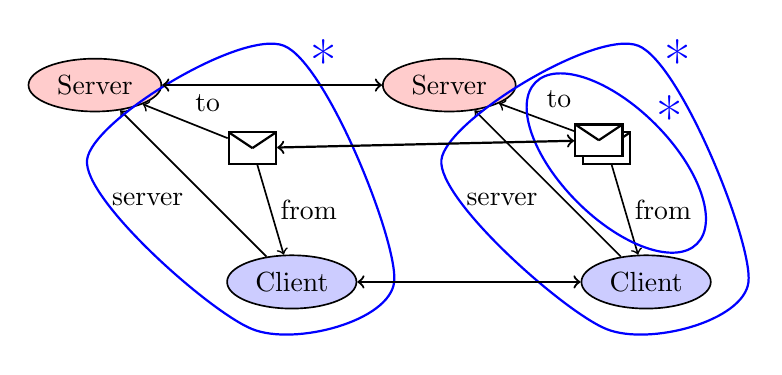
\begin{tikzpicture}[semithick, ->, node distance=2cm]

  \visible<2->{
  \begin{scope}
    \node [draw,ellipse,fill=red!20]  (x) at ( 0, 0) {Server};
    \node [draw,ellipse,fill=blue!20] (m) at ( 2.5, -2.5) {Client};
    \path  (m) edge node [below left] {server} (x);
    \tikzMessageNode{mm}{2.0,-0.8}
    \path  (mm) edge node [right] {from} (m);
    \path  (mm) edge node [above right] {to} (x);
    \draw[color=blue,thick] plot[smooth cycle] coordinates{(-0.1,-0.95) (2.4,0.5) (3.8,-2.5) (2,-3.1)};
    \node[text=blue] (star) at ( 2.9, 0.3) {{\huge *}};
  \end{scope}
  }
 
  \begin{scope}[xshift=4.5cm]
    \node [draw,ellipse,fill=red!20]  (x2) at ( 0, 0) {Server};
    \node [draw,ellipse,fill=blue!20] (m2) at ( 2.5, -2.5) {Client};
    \path  (m2) edge node [below left] {server} (x2);
    \tikzMessageNode{mm1}{2.0,-0.8}
    \tikzMessageNode{mm2}{1.9,-0.7}
    \path  (mm1) edge node [right] {from} (m2);
    \path  (mm2) edge node [above right] {to} (x2);
    \draw[color=blue,thick] plot[smooth cycle] coordinates{(-0.1,-0.95) (2.4,0.5) (3.8,-2.5) (2,-3.1)};
    \node[text=blue] (star) at ( 2.9, 0.3) {{\huge *}};
    \visible<4->{
      \draw[thick,rotate=45,color=blue] (0.8,-2.2) ellipse (0.7 and 1.45);
      \node[text=blue] (star) at ( 2.8, -0.4) {{\huge *}};
    }
  \end{scope}
  
  \visible<3->{
    \path[<->,thick] (x) edge (x2);
    \path[<->,thick] (m) edge (m2);
    \path[<->,thick] (mm) edge (mm2);
  }

  \end{tikzpicture}
  \end{figure}
\end{frame}

\begin{frame}
  \frametitle{How the Covering Set Grows ?}
    \begin{table}[t]
    \centering
    {\footnotesize
    \begin{tabular}{|l|r|r|r|}
    \hline
    Name &  tree size & cov.~set size & time \\
    \hline
    \hline
    \texttt{ping-pong} & 17 & 14 & 0.6\,s \\
    \hline
    \texttt{client-server} & 25 & 2 & 1.9\,s \\
    \hline
    \texttt{client-server-with-TO} & 184 & 5 & 12.8\,s \\
    \hline
    \texttt{genericComputeServer} & 57 & 4 & 4.6\,s \\
    \hline
    \texttt{genericComputeServer-fctAsActor} & 98 & 8 & 14.8\,s \\
    \hline
    \texttt{liftChatLike} & 1846 & 21 & 1830.9\,s \\
    \hline
    \texttt{round\_robin\_2} & 830 & 63 & 48.8\,s \\
    \hline
    \texttt{round\_robin\_3} & 3775 & 259 &  737.8\,s \\
    \hline 
    \end{tabular}
    \\ [1ex]
    }
    \caption{Experimental results: the columns indicate the number of
      nodes in the Karp-Miller tree, the number of ideals in
      the covering set, and the running time.}
    \label{tbl:xp-results}
    \end{table}
\end{frame}

\begin{frame}
  \frametitle{Interesting Properties of the Cover}

  The covering set:
  \begin{itemize}
  \item can answer an covering question (control-state reachability),
  \item has a compact representation,
  \item is an inductive invariant.
  \end{itemize}

  The first point was the original motivation for this work.

  The last two points allows us to do much more.

  \vspace{2ex}

  Show \picasso output for the client-server example.

  \picasso is available at \url{http://pub.ist.ac.at/~zufferey/picasso/}.
\end{frame}

%\begin{frame}
%  \frametitle{Further related work:}

%  \begin{description}
%  \item[\cite{DBLP:conf/lics/AbdullaCJT96}]
%  Complete backward algorithm for coverability
%  \item[\cite{GeeraertsETAL06ExpandEnlargeCheck}]
%  Complete algorithm for coverability based on ideal completions  
%  \item[\cite{DBLP:conf/vmcai/GantyRB06}]
%  Complete algorithm for coverability based on abstract interpretation but not ideal completions
%  \item[\cite{FinkelGoubaultLarrecq09ForwardAnalysisForWSTS}]
%  Acceleration-based algorithm for computing covering sets
%  \end{description}

%\end{frame}

%\begin{frame}
%  \frametitle{Conclusion}
%  \begin{itemize}
%  \item Many verification problems for concurrent systems can be phrased in terms of coverability
%  \item Coverability is decidable for well-structured transition systems but with high complexity
%  \item \alert{Ideal Abstraction}: a generic framework for computing an approximation of the covering set.
%    \begin{itemize}
%    \item promises precise but more scalable analysis of WSTS
%    \item we provide instantiations of the framework for common classes of WSTS
%    \item \alert{Picasso}: implementation of our framework for the analysis of Scala actor programs
%    \end{itemize}
%  \end{itemize}
%\end{frame}

\section{Using the Covering Set}

\subsection{Termination of DBS}

\begin{frame}
  \frametitle{Termination Proofs and Counter Abstractions}
  Termination proof:\\
  \mbox{}~~finite union of ranking function \cite{transinv}\\

  \vspace{1ex}

  Counter abstraction:\\
  \mbox{}~~counts the number of occurrences of some elements in a system.
  Typically one counts the number of processes in a state/control-location.

  \vspace{1ex}

  In this work we automatically infer complex termination proof using a flexible counter abstraction.
  The number of counters is not fixed a priori, but depends on the reachable states in the system.
  This is joint work with Kshitij Bansal, Eric Koskinen, and Thomas Wies (just rejected from POPL).
\end{frame}

\begin{frame}[fragile]
  \frametitle{Treiber's stack: code}
  \begin{columns}
    \column{0.5\linewidth}
{\footnotesize
\begin{verbatim}
struct node {
    struct node *next;
    value data;
};
struct stack { struct node *Top; };
struct stack *S;

value pop() {
  struct node *t, *x;
  do {
    t = S->Top;
    if (t == NULL) return EMPTY;
    x = t->next;
  } while (!CAS(&S->Top,t,x));
  return t->data;
}
\end{verbatim}
}
    \column{0.5\linewidth}
{\footnotesize
\begin{verbatim}
  void init() {
      S = alloc();
      S->Top = NULL;
  }


  void push(value v) {
    struct node *t, *x;
    x = alloc();
    x->data = v;
    do {
        t = S->Top;
        x->next = t;
    } while (!CAS(&S->Top,t,x));
  }
\end{verbatim}
}
  \end{columns}

\end{frame}

\begin{frame}
  \frametitle{Treiber's stack: as DBS and Covering Set}
  Encoding:
  \begin{itemize}
  \item {\tt push} and {\tt pop} are a single operation.
  \item Operation: first read the top of stack, then CAS.
  \end{itemize}

  \vspace{2ex}

  Invariant for termination:\\
  A process cannot fail twice unless someone else did succeed. 
  
  \vspace{2ex}

  \begin{center}
  Show \picasso output: rewrite rules, cover, and cover + post.
  \end{center}

\end{frame}

\begin{frame}
  \frametitle{Numerical Abstraction from the Covering Set}
  % goes back to what ideals represents
  % associate a counter to each node in the graph

  \begin{minipage}{6cm}
  Op2: CAS succeed

  \scalebox{0.75}{
  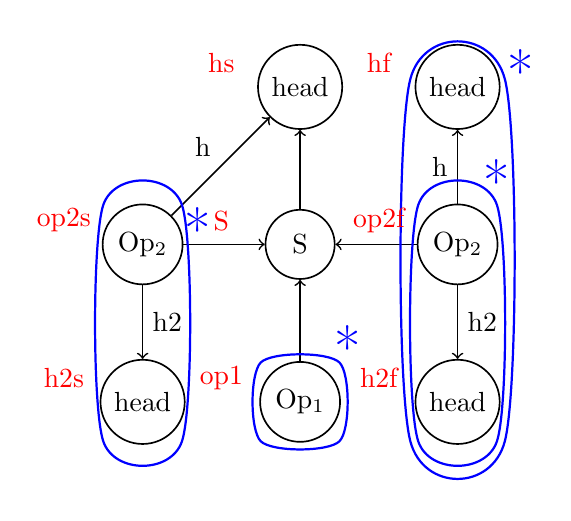
\begin{tikzpicture}[->,auto, node distance=20mm, semithick]
    \node [state] (s) {S};
    \node [state] (op1) [below of=s] {Op$_1$};
    \node [state] (op2s) [left of=s] {Op$_2$};
    \node [state] (op2f) [right of=s] {Op$_2$};
    \node [state] (hs) [above of=s] {head};
    \node [state] (hf) [above of=op2f] {head};
    \node [state] (h2s) [below of=op2s]  {head};
    \node [state] (h2f) [below of=op2f] {head};
    \path
    (s) edge (hs)
    (op1) edge (s)
    (op2s) edge (s)
    (op2f) edge (s)
    (op2s) edge node {h} (hs)
    (op2f) edge node {h} (hf)
    (op2s) edge node {h2} (h2s)
    (op2f) edge node {h2} (h2f)
    %(pi1) edge [bend left] node[right] { \_ ? Pong } (pi2)
    %(pi2) edge [bend left] node[left] { actor$_{pong}$ ! Ping } (pi1)
    %(pi2) edge [bend right] node[below] { actor$_{pong}$ ! Stop } (pi3)
    ;
    \draw[color=blue,thick] plot[smooth cycle] coordinates{(0.5,-1.5) (0.5,-2.5) (-0.5,-2.5) (-0.5,-1.5)};
    \node[text=blue] (star) at ( 0.6, -1.3) {{\huge *}};
    \draw[color=blue,thick] plot[smooth cycle] coordinates{(-1.5,0.5) (-2.5,0.5) (-2.5,-2.5) (-1.5,-2.5)};
    \node[text=blue] (star) at ( -1.3, 0.2) {{\huge *}};
    \draw[color=blue,thick] plot[smooth cycle] coordinates{(1.5,0.5) (2.5,0.5) (2.5,-2.5) (1.5,-2.5)};
    \node[text=blue] (star) at ( 2.5, 0.8) {{\huge *}};
    \draw[color=blue,thick] plot[smooth cycle] coordinates{(1.4,2.1) (2.6,2.1) (2.6,-2.5) (1.4,-2.5)};
    \node[text=blue] (star) at ( 2.8, 2.2) {{\huge *}};
    
    \visible<2->{
    \node [red] (cs) at (-1,0.3) {S};
    \node [red] (cop1) [below of=cs] {op1};
    \node [red] (cop2s) [left of=cs] {op2s};
    \node [red] (cop2f) [right of=cs] {op2f};
    \node [red] (chs) [above of=cs] {hs};
    \node [red] (chf) [above of=cop2f] {hf};
    \node [red] (ch2s) [below of=cop2s]  {h2s};
    \node [red] (ch2f) [below of=cop2f] {h2f};
    }
  \end{tikzpicture}
  }
  \end{minipage}
  \begin{minipage}{3cm}
  \includegraphics[scale=0.35]{op2_success}
  \end{minipage}

  \visible<3->{
  \parbox{2.5cm}{
    S' = S\\
    op1' = op1\\
    op2s' = 0
  }
  \parbox{5cm}{
    op2f' = op2f + op2s -1\\
    h2f' = h2f + h2s - 1\\
    hf' = hf + 1
  }
  \parbox{2.5cm}{
    hs' = 1 \\
    h2s' = 0
  }
  }

\end{frame}

\begin{frame}
  \frametitle{Theoretical results}

  Soundness:\\
  \mbox{}~~The numerical abstraction preserves the weak-fair termination.

  \vspace{2ex}

  Preserving Monotonicity:\\
  \mbox{}~~The numerical abstraction preserves the monotonicity of the DBS.
  The numerical abstraction is actually a Petri Net.

\end{frame}

\begin{frame}
  \frametitle{Implementation}

\begin{table}[t]
\begin{center}
\begin{small}
\begin{tabularx}{\linewidth}{l>{\raggedleft}X>{\raggedleft}X>{\raggedleft}X>{\raggedleft\arraybackslash}X}
\toprule
\multirow{2}{*}{\bf Example} & {\bf Cov} & {\bf Cov}+$\mathcal{N}$ & {\bf ARMC} &{\bf Total}\\
& {\bf size} & (sec) & (sec) & (sec)\\
\midrule
\texttt{split/merge}             &  3 &   3.5   &  4.5   & 8.0 \\
Work stealing, 3 processors      &  3 &   5.4   &  1.0   & 6.4 \\
Parameterized work stealing      &  1 &   3.7   &  0.9   & 4.6 \\
Compute server job queue         &  1 &   3.9   &  1.2   & 5.1 \\
Map reduce                       &  4 &   5.6   &  0.9   & 6.5 \\
Map reduce with failure          &  5 &   7.9   &  6.0   & 13.9 \\
Treiber's stack                  &  1 &   3.8   &  0.5   &  4.3 \\
Treiber's stack (fine-grained)   &  3 &  10.3   &  4.7   & 15.0 \\
Herlihy Wing queue               &  2 &  20.4   &  85.9  & 106.3 \\
\bottomrule
\end{tabularx}
\\ [1ex]
\end{small}
\end{center}
\caption{Experimental results. Columns indicate the size of the
  cover, the running time for its construction and the construction of the numerical abstraction,
  the running time of the final termination, and the total time of our method.}
\label{tbl:xp-results}
\end{table}

\end{frame}

\subsection{Dynamic Package Interface}

\begin{frame}
  \frametitle{Object Interfaces}
  Example: 
  one should invoke the lock and unlock methods of a lock object in alternation, starting by lock.
  \begin{center}
    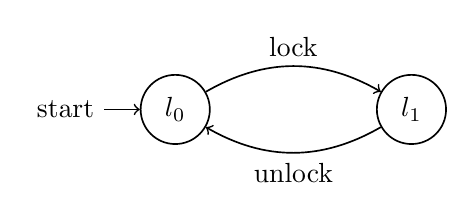
\begin{tikzpicture}[->,auto, node distance=3cm, semithick]
      \node [state,initial] (pi0) {$l_0$};
      \node [state] (pi1) [right of=pi0] {$l_1$};
      \path
      (pi0) edge [bend left] node { lock } (pi1)
      (pi1) edge [bend left] node { unlock } (pi0)
      ;
    \end{tikzpicture}
  \end{center}

  \vspace{2ex}

  In this work we use the covering set to extract interface for \emph{groups of objects} in a non-concurrent setting.
  This is joint work with Shahram Esmaeilsabzali, Rupak Majumdar, and Thomas Wies (submitted to ICSE).
\end{frame}

\begin{frame}[fragile]
  \frametitle{Example: Sets and Iterators}
  \begin{columns}
    \column{0.5\linewidth}
{\footnotesize
\begin{verbatim}
class Set {
  protected int sver, size;
  public Set() {
    sver := size := 0;
  }
  public void add(int elem) {
    if (!duplicate) {
      sver++; size++;
    }
  }
  protected void delete(int pos) {
    sver++; size--;
  }
  public Iterator iterator() {
    return (new Iterator(this));
  }
}
\end{verbatim}
}
    \column{0.5\linewidth}
{\footnotesize
\begin{verbatim}
class Iterator {
  int iver, pos;
  Set it_of;
  protected Iterator(Set s) {
    it_of := s; pos := 0;
    iver := s.sver;
  }
  public int next() {
    if (iver == S.sver) then pos++;
    else throw new Exception();
  }
  public void remove() {
    if (iver == S.sver) then {
      it_of.delete(pos);
      iver := S.sver;
    } else {
      throw new Exception();
} } }
\end{verbatim}
}
  \end{columns}

\end{frame}

\begin{frame}
  \frametitle{Predicate Abstraction and DBS Encoding}
  How do we get from the code to the DBS ?

  We use predicates abstraction and symbolic execution.
  \begin{itemize}
  \item unary predicate for {\tt Set}:\\
    empty ({\tt size = 0})
  \item binary predicates for {\tt Set} and {\tt Iterator}:\\
    sync ({\tt iver = it\_of.sver})
  \end{itemize}

\end{frame}

\begin{frame}
  \frametitle{Rewriting rule for {\tt Iterator.remove}}
  %Assume that the iterator lies in the bounds of the collection and that the set is not empty.
    
  We have to consider a few cases:
  \begin{itemize}
  \item An iterator can be either synchronized or not.
  \item An iterator can be either the caller or part of the frame.
  \end{itemize}

  \scalebox{0.8}{
  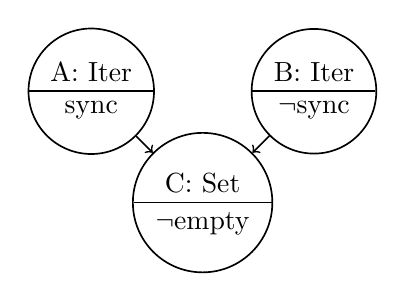
\begin{tikzpicture}[->,auto, node distance=20mm, semithick]
    \node [draw,circle split] (s) {C: Set \nodepart{lower} $\neg$empty};
    \node [draw,circle split] (it1) [above right of=s] {B: Iter \nodepart{lower} $\neg$sync};
    \node [draw,circle split] (it2) [above left of=s] {A: Iter \nodepart{lower} sync};
    \path
    (it1) edge (s)
    (it2) edge (s)
    ;
  \end{tikzpicture}
  }
  \begin{minipage}[b]{5cm}
  \begin{eqnarray*}
    \varphi(A,A) & \Rightarrow & wp(\text{$A$.remove}, \text{sync}_{A'}) \\
    \varphi(A,A) & \Rightarrow & wp(\text{$A$.remove}, \neg\text{sync}_{A'}) \\
    \varphi(B,A) & \Rightarrow & wp(\text{$A$.remove}, \text{sync}_{B'}) \\
    \varphi(B,A) & \Rightarrow & wp(\text{$A$.remove}, \neg\text{sync}_{B'}) \\
    \varphi(C,A) & \Rightarrow & wp(\text{$A$.remove}, \text{empty}_{C'}) \\
    \varphi(C,A) & \Rightarrow & wp(\text{$A$.remove}, \neg\text{empty}_{C'})
  \end{eqnarray*}
  \end{minipage}

  \vspace{2ex}

  To know what cases we must consider, we go back and forth between the cover computation and the symbolic execution.

\end{frame}

\begin{frame}
  \frametitle{Extracting the DPI}
  \begin{itemize}
  \item compute the covering set and the DBS
  \item apply the post operator once more
  \item track each transition to get the DPI
  \end{itemize}

  \vspace{2ex}

  Show \picasso output for the Set and Iterators example.
\end{frame}

\section*{Conclusion}

\begin{frame}
  \frametitle{Conclusion}

  We present an analysis to compute an over-approximation of the covering set for BDS.

  Then we show that on top of answering coverability question the covering set can be used as starting point for more advanced analysis:
  \begin{itemize}
  \item numerical abstraction to prove (weak-fair) termination;
  \item interfaces for groups of objects.
  \end{itemize}

\end{frame}


\begin{frame}[allowframebreaks]{References}
  \frametitle{}
  {\tiny
  %\bibliographystyle{annotate}
  %\bibliographystyle{plainnat}
  \bibliographystyle{cell}
  %\bibliographystyle{abbrvnat}
  \bibliography{biblio}
  }
\end{frame}

\end{document}
